% Provenance (never printed): sources/book2/BRIEFS.md, g11-13. A bank's balance sheet; loans create deposits; the money
% multiplier as a toy model and its failure after 2008; the central bank and the policy rate; runs, deposit insurance and
% capital. Real numbers: figdata/grade-11/13-money-and-banking/ (JST narrow and broad money, USA 2000-2020). Ledger: Bank of
% England 2014, FDIC limit, Banking Act 1933, Federal Reserve History on the 1930-31 panics, BIS capital buffer. The Basel
% minimum ratios were not found on the pages read and are not printed. Photograph: a 1931 bank run (Commons, PD). Brenland's
% banks are invented.
\chapter{Money and Banking}\label{ch:g11:money-and-banking}

In 2007 the narrow money of the United States, essentially the money issued by its central bank, was 847 billion dollars. By 2019 it was 3426 billion, four times as
much. \omterm{def:g11:money-and-banking:broad-money}{Broad money}, mostly the deposits that people and firms hold at banks, grew from 7294 billion to 14\,836 billion: it doubled. From 1995 to 2007 \omterm{def:g11:money-and-banking:broad-money}{broad money} was
about eight times narrow money (since 1950 the ratio had ranged from about 5 to 11); after 2008 it fell to under five.
% figdata: usa_money (2007 847, 7294, ratio 8.6; 2019 3426, 14836, ratio 4.3); usa_ratio_long (1950 5.4, 1960 7.7, 1970 9.1, 1980 10.9, 1985 11.4, 1990 10.6, 1995 7.8, 2005 8.0, 2010 4.3)

A textbook model said that \omterm{def:g11:money-and-banking:broad-money}{broad money} is a fixed multiple of \omterm{def:g11:money-and-banking:reserves}{central bank money}. This chapter shows where that model comes from, why it broke, and how money is really
made: mostly by banks, when they lend. It then turns to what can go wrong with banks, and to the rules built after it did.

\begin{openingchart}{United States, 2000--2020. Left: narrow money (as the Macrohistory Database defines it, close to the central bank's monetary base) and broad money,
index 2000 = 100. Right: broad money divided by narrow money.}{Jordà--Schularick--Taylor Macrohistory Database}
\begin{tikzpicture}
\begin{groupplot}[group style={group size=2 by 1, horizontal sep=1.5cm}, omtime, height=5.0cm, xmin=2000, xmax=2020, xtick={2000,2005,...,2020}]
\nextgroupplot[omtime, width=0.5\linewidth, ymin=0, ymax=900, ylabel={index, 2000 = 100}]
\addplot[omThm, thick] table[x=year, y=narrow_idx] {figdata/grade-11/13-money-and-banking/out/usa_money.csv};
\addplot[omDef, thick] table[x=year, y=broad_idx] {figdata/grade-11/13-money-and-banking/out/usa_money.csv};
\node[omThm, font=\scriptsize, anchor=east] at (axis cs:2010,560) {narrow money};
\node[omDef, font=\scriptsize, anchor=west] at (axis cs:2010,170) {broad money};
\nextgroupplot[omtime, width=0.4\linewidth, ymin=0, ymax=10, ylabel={broad / narrow}]
\addplot[black, thick] table[x=year, y=ratio] {figdata/grade-11/13-money-and-banking/out/usa_money.csv};
\end{groupplot}
\end{tikzpicture}
\end{openingchart}

\begin{recall}
From the grades 6--9 volume: money as a means of payment, a unit of account and a store of value; banks, deposits, loans and interest. From
\cref{ch:g11:asymmetric-information}: \omterm{def:g11:asymmetric-information:moral-hazard}{moral hazard}. From the mathematics volumes: the sum of a geometric series, $1 + q + q^2 + \dots = 1/(1 - q)$ for $|q| < 1$.
\end{recall}

\section{A bank's balance sheet}\label{sec:g11:money-and-banking:balance-sheet}

\begin{definition}[Balance sheet and bank capital]\label{def:g11:money-and-banking:balance-sheet}
A \emph{balance sheet}\index{balance sheet} lists, at a date, what an organisation owns (its assets) and what it owes (its liabilities). A bank's \emph{bank capital}\index{bank
capital}\phantomsection\label{def:g11:money-and-banking:bank-capital} is its assets minus its liabilities: what would be left for its owners if every asset were sold at its
recorded value and every debt paid.
\end{definition}

\begin{definition}[Reserves and central bank money]\label{def:g11:money-and-banking:reserves}
A bank's \emph{reserves}\index{reserves} are the deposits it holds at the central bank, plus its cash. \emph{Central bank money}\index{central bank money}%
\phantomsection\label{def:g11:money-and-banking:central-bank-money} is the money the central bank issues: notes and coins, and banks' reserves at the central bank.
\end{definition}

\begin{definition}[Broad money]\label{def:g11:money-and-banking:broad-money}
\emph{Broad money}\index{broad money} is the money held by households and firms: notes and coins in their hands, and their deposits at banks.
\end{definition}

A bank's assets are its \omterm{def:g11:money-and-banking:reserves}{reserves}, its loans and the bonds it holds; its liabilities are mainly its customers' deposits. Capital is the cushion between them: a bank with
assets of 220 and deposits of 200 has capital of 20, and can lose 20 on its assets before it owes more than it owns.

\section{Loans create deposits}\label{sec:g11:money-and-banking:creation}

\begin{definition}[Money creation]\label{def:g11:money-and-banking:money-creation}
\emph{Money creation}\index{money creation} is the increase in \omterm{def:g11:money-and-banking:broad-money}{broad money} that happens when a bank makes a loan and credits the borrower's account with a new deposit.
Money is destroyed when a loan is repaid out of a deposit.
\end{definition}

\begin{omfigure}
\renewcommand{\arraystretch}{1.25}
\begin{tabular}{l|r@{\hspace{2.5em}}l|r}
\multicolumn{4}{c}{\textbf{Bank A: a loan of 10 to a baker}} \\
\multicolumn{2}{c|}{assets} & \multicolumn{2}{c}{liabilities} \\ \hline
loans & $+10$ & deposit of the baker & $+10$ \\
\end{tabular}

\medskip
\begin{tabular}{l|r@{\hspace{2.5em}}l|r}
\multicolumn{4}{c}{\textbf{The baker pays a miller at bank B}} \\
\multicolumn{2}{c|}{assets} & \multicolumn{2}{c}{liabilities} \\ \hline
A: \omterm{def:g11:money-and-banking:reserves}{reserves} & $-10$ & A: deposit of the baker & $-10$ \\
B: \omterm{def:g11:money-and-banking:reserves}{reserves} & $+10$ & B: deposit of the miller & $+10$ \\
\end{tabular}

\medskip
{\small T-accounts of a loan. The loan creates a deposit of 10, new money, with a stroke of the pen (top). When the baker spends it, the deposit moves to bank B, and bank A
settles by transferring 10 of \omterm{def:g11:money-and-banking:reserves}{reserves} at the central bank (bottom). \omterm{def:g11:money-and-banking:broad-money}{Broad money} has risen by 10; \omterm{def:g11:money-and-banking:reserves}{central bank money} has not changed.}
\end{omfigure}

What limits lending, then, is not the deposits a bank already has but whether it can find borrowers it trusts at the interest rate it charges, whether it has enough capital,
and the rate at which it can borrow \omterm{def:g11:money-and-banking:reserves}{reserves} when payments flow out. A study by the Bank of England put it plainly: most money is created by commercial banks making loans,
banks do not \emph{multiply up} \omterm{def:g11:money-and-banking:reserves}{central bank money}, and how much money they create depends in the end on the central bank's policy.
% ledger: g11:boe2014

\begin{measure}[Measures of money]
\omterm{def:g11:money-and-banking:reserves}{Central bank money} (the \emph{monetary base}) is notes and coins plus banks' \omterm{def:g11:money-and-banking:reserves}{reserves} at the central bank. Narrow money adds to the notes and coins in circulation the
deposits that can be spent at once. \omterm{def:g11:money-and-banking:broad-money}{Broad money} adds savings deposits and other near-money. Each country defines its measures in detail, so comparisons across countries
use the definitions of one source. The series called narrow money in the opening chart is the database's own; for the United States it moves
with the monetary base, not with the narrow money defined here, so the chart's ratio stands for \omterm{def:g11:money-and-banking:broad-money}{broad money} over \omterm{def:g11:money-and-banking:reserves}{central bank money}.
\end{measure}

\section{The money multiplier, a toy model}\label{sec:g11:money-and-banking:multiplier}

\begin{definition}[Money multiplier]\label{def:g11:money-and-banking:money-multiplier}
The \emph{money multiplier}\index{money multiplier} is the ratio of \omterm{def:g11:money-and-banking:broad-money}{broad money} to \omterm{def:g11:money-and-banking:reserves}{central bank money}.
\end{definition}

\begin{proposition}[The multiplier of the toy model]\label{prop:g11:money-and-banking:multiplier}
Suppose the public holds cash equal to a share $c$ of its deposits, banks hold \omterm{def:g11:money-and-banking:reserves}{reserves} equal to a share $r$ of deposits and lend the rest, and \omterm{def:g11:money-and-banking:reserves}{central bank money} is $B$.
Then deposits are $D = B/(c + r)$, \omterm{def:g11:money-and-banking:broad-money}{broad money} is $M = (1 + c)D$, and the multiplier is $M/B = (1 + c)/(c + r)$.
\end{proposition}
\begin{proof}
\omterm{def:g11:money-and-banking:reserves}{Central bank money} is held either as cash by the public or as \omterm{def:g11:money-and-banking:reserves}{reserves} by banks: $B = cD + rD$, so $D = B/(c + r)$. \omterm{def:g11:money-and-banking:broad-money}{Broad money} is cash plus deposits, $cD + D = (1 + c)D$.
The same result comes as a geometric sum: a new unit of \omterm{def:g11:money-and-banking:reserves}{central bank money} ends up partly as cash and partly as \omterm{def:g11:money-and-banking:reserves}{reserves}; at each round, banks lend the part of new deposits
they do not keep, a fraction $q = 1/(1 + c) \times (1 - r)$ of it returns as a new deposit, and the deposits created add up to $1 + q + q^2 + \dots = 1/(1 - q)$ times the
first.
\end{proof}

\begin{model}{The money multiplier (toy)}
\assumes Banks lend every reserve beyond the share $r$ they keep; the public holds a fixed share $c$ of its money in cash.
\predicts \omterm{def:g11:money-and-banking:broad-money}{Broad money} moves in proportion to \omterm{def:g11:money-and-banking:reserves}{central bank money}: the central bank sets the quantity of money through $B$.
\tested Consistent with it, roughly, in years when banks held few excess \omterm{def:g11:money-and-banking:reserves}{reserves}; in the United States the ratio of broad to narrow money was 7.8 in 2000 and 8.6 in 2007.
\breaks After 2008, when the central bank quadrupled its money and banks held the new \omterm{def:g11:money-and-banking:reserves}{reserves} instead of lending them: the ratio fell to 2.9 by 2014. When \omterm{def:g11:money-and-banking:reserves}{reserves} earn
  interest and good borrowers are scarce, banks need not lend \omterm{def:g11:money-and-banking:reserves}{reserves} out.
\end{model}
% figdata: usa_money (ratio 2000 7.8, 2007 8.6, 2014 2.9)

\section{The central bank}\label{sec:g11:money-and-banking:central-bank}

\begin{definition}[Policy rate]\label{def:g11:money-and-banking:policy-rate}
The \emph{policy rate}\index{policy rate} is the short-term interest rate that the central bank sets and steers, at which banks borrow or lend \omterm{def:g11:money-and-banking:reserves}{reserves} overnight.
\end{definition}

The central bank is the bank of the banks: payments between banks are settled in \omterm{def:g11:money-and-banking:reserves}{reserves} held with it. It steers the overnight rate by paying interest on \omterm{def:g11:money-and-banking:reserves}{reserves} and
by lending \omterm{def:g11:money-and-banking:reserves}{reserves} at a rate a little above that: no bank lends \omterm{def:g11:money-and-banking:reserves}{reserves} to another for less than the central bank pays, and none borrows for more than the central bank
charges. Through that rate it influences the rates at which banks lend, and so how much they lend and how much money they create. Later chapters return to what it aims at.

\section{Runs, insurance and capital}\label{sec:g11:money-and-banking:runs}

\begin{definition}[Bank run]\label{def:g11:money-and-banking:bank-run}
A \emph{bank run}\index{bank run} occurs when many depositors try to withdraw their deposits at once, for fear that the bank will fail.
\end{definition}

A bank lends long and borrows short: its loans are repaid over years, but its deposits can be withdrawn today. If all depositors ask for their money, the bank must sell
loans quickly and at a loss. So a run can make a sound bank fail: each depositor is right to run if the others run, and right to stay if they stay.

\begin{omfigure}
\renewcommand{\arraystretch}{1.3}
\begin{tabular}{lcc}
\toprule
 & other depositor stays & other depositor runs \\
\midrule
you stay & 110, 110 & 50, 100 \\
you run & 100, 50 & 75, 75 \\
\bottomrule
\end{tabular}

{\small A \omterm{def:g11:money-and-banking:bank-run}{bank run} as a \omterm{def:g11:oligopoly-and-games:game}{game} between two depositors of 100 each (your \omterm{def:g11:oligopoly-and-games:game}{payoff} first). If both wait, the bank's loans pay 110 each. A depositor who runs alone gets 100; the
bank then sells loans at a loss and the one who stayed gets 50. If both run, the fire sale leaves 75 each. Both staying and both running are equilibria.}
\end{omfigure}

\begin{model}{A bank run as a coordination game}
\assumes Deposits can be withdrawn at any time; loans can be sold quickly only at a loss; each depositor acts on what she expects the others to do.
\predicts Two equilibria: no run, and a run that brings the bank down whatever its loans are worth; a rumour can move depositors from one to the other.
\tested Consistent with the waves of bank suspensions in the United States from 1930 to 1933, in which hundreds of banks closed within a few weeks
  (see the record below); how many of the banks that failed were sound, and so how many failures the runs themselves caused, is still argued over.
\breaks When deposits are insured, so that no insured depositor gains by running; when a central bank stands ready to lend to sound banks against their loans.
\end{model}

\begin{definition}[Deposit insurance and lender of last resort]\label{def:g11:money-and-banking:deposit-insurance}
\emph{Deposit insurance}\index{deposit insurance} is a guarantee, usually by a public agency, that depositors will be repaid up to a limit if their bank fails. A
\emph{lender of last resort}\index{lender of last resort}\phantomsection\label{def:g11:money-and-banking:lender-of-last-resort} is a central bank that lends to banks
short of cash, against good collateral, when no one else will.
\end{definition}

\begin{record}[Bank runs in the United States, 1930--33]
% ledger: g11:panics-1930, g11:ba1933, g11:fdic-limit
When the crises began, nearly 16\,000 American banks were outside the Federal Reserve System and over 8000 inside it. In November 1930, hundreds of banks suspended
operations within a few weeks; about a third reopened, most were wound up. On 11 December 1930 the Bank of United States, the fourth-largest bank in New York City, closed;
a new crisis broke out in Chicago in June 1931, and suspensions peaked in 1933. The Banking Act, signed on 16 June 1933, created the Federal Deposit Insurance Corporation;
insurance began in January 1934, at first up to 2500 dollars per account holder. Since 1934, no depositor has lost insured funds.
\end{record}

\begin{omfigure}
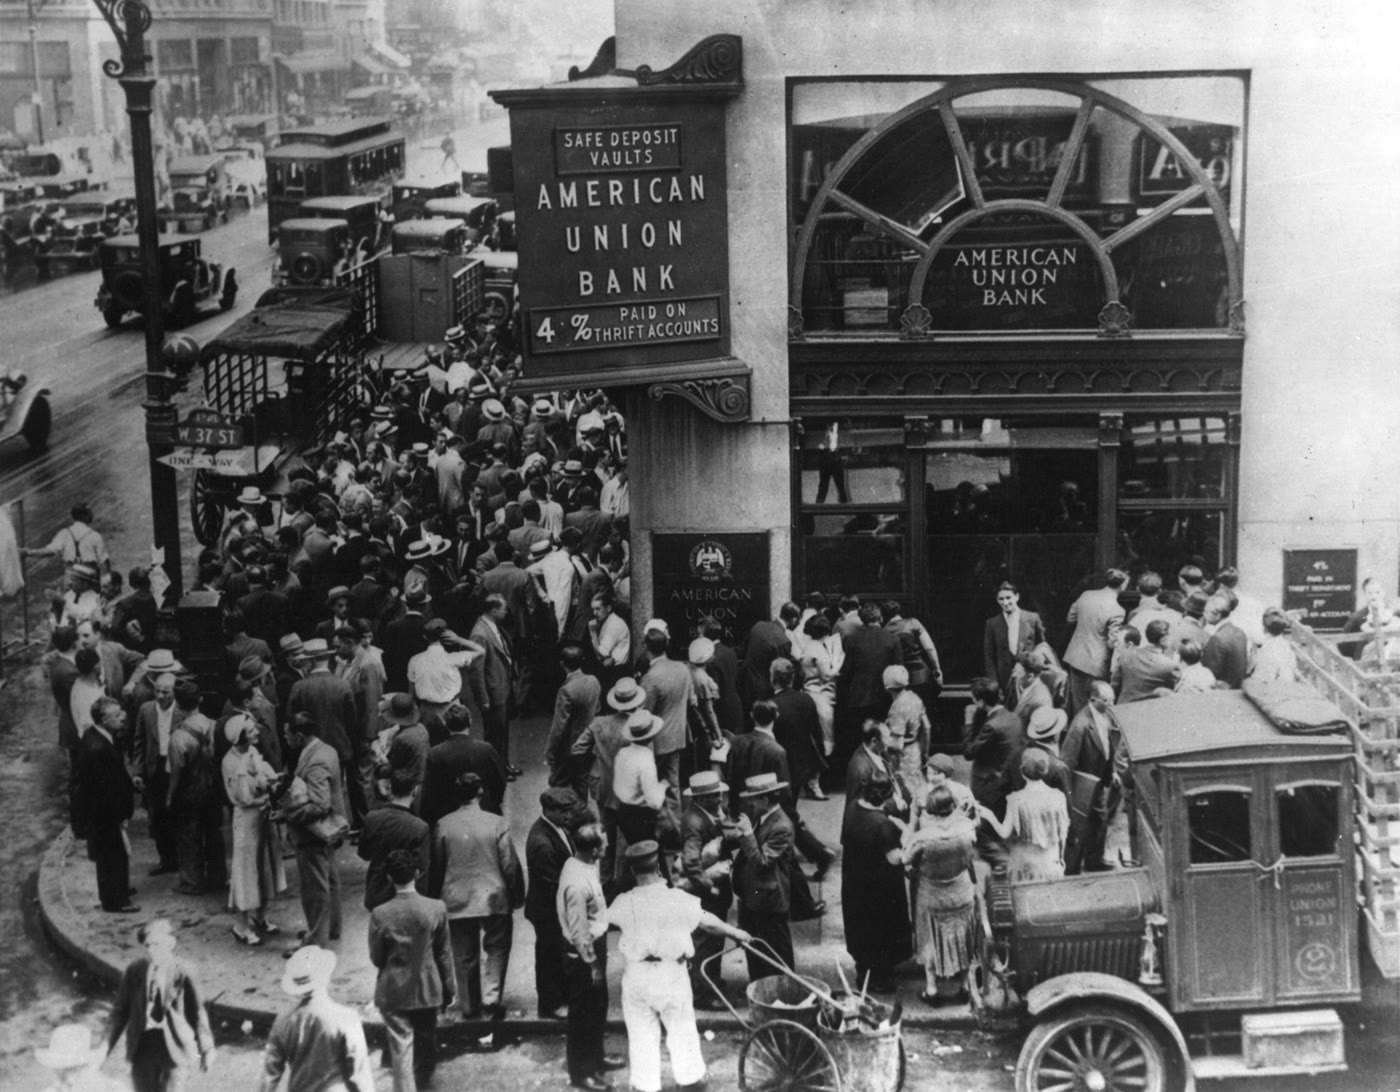
\includegraphics[width=0.58\linewidth]{images/book2/photos/g11-banking-bank-run-1931.jpg}

{\small A crowd outside the American Union Bank in New York, 1931. The bank, opened in 1917, closed on 30 June 1931.}
\end{omfigure}

Insurance stops runs, but it creates \omterm{def:g11:asymmetric-information:moral-hazard}{moral hazard}: insured depositors no longer watch what their bank does with their money, and a bank's owners, who lose only their
capital if a gamble fails, gain from taking more risk. Rules on capital answer that. There are private answers too. A bank can hold more
capital or more liquid assets than any rule requires; a bank funded far more by its owners' shares than by deposits that can be withdrawn at any
time has much less to fear from a run; and large depositors who are not insured have a reason to watch it. Before \omterm{def:g11:money-and-banking:deposit-insurance}{deposit
insurance}, some banks' contracts let them delay withdrawals in a panic, and American banks in a city joined in clearing houses that lent to their
members when runs began; these answers worked in some panics and failed in others. And a guarantee can breed the risk it insures: when
depositors and lenders expect a large bank to be rescued in full, they stop watching it.

\begin{definition}[Capital ratio]\label{def:g11:money-and-banking:capital-ratio}
A bank's \emph{capital ratio}\index{capital ratio} is its capital divided by its assets, each asset weighted by its risk (a loan to a firm counts more than a
government bond).
\end{definition}

\begin{dated}{2026}
% ledger: g11:fdic-limit, g11:basel-buffer
American \omterm{def:g11:money-and-banking:deposit-insurance}{deposit insurance} covers up to 250\,000 dollars per depositor, per insured bank, for each kind of account ownership. The international banking rules require,
above each bank's minimum \omterm{def:g11:money-and-banking:capital-ratio}{capital ratios}, a further buffer of the highest-quality capital equal to 2.5\,\% of its risk-weighted assets.
\end{dated}

\section{Exercises}

\begin{exercise}[$\star$]\label{exo:g11:money-and-banking:1}
A household deposits 500 dalens of notes at its bank, which holds them as cash. Write the bank's T-account.
\end{exercise}

\begin{exercise}[$\star$]\label{exo:g11:money-and-banking:2}
A bank lends 1000 dalens to a firm and credits its account. Write the T-account. Has \omterm{def:g11:money-and-banking:broad-money}{broad money} changed?
\end{exercise}

\begin{exercise}[$\star$]\label{exo:g11:money-and-banking:3}
A bank buys a bond worth 200 from a household and pays by crediting the household's deposit. Write the T-account. Has \omterm{def:g11:money-and-banking:broad-money}{broad money} changed?
\end{exercise}

\begin{exercise}[$\star$]\label{exo:g11:money-and-banking:4}
From the opening chart and the figures in the text, by what factor did narrow money grow from 2007 to 2019, and \omterm{def:g11:money-and-banking:broad-money}{broad money}?
\end{exercise}

\begin{exercise}[$\star$]\label{exo:g11:money-and-banking:5}
A bank has assets of 500 and capital of 40. Compute its \omterm{def:g11:money-and-banking:capital-ratio}{capital ratio} (unweighted) and its deposits, if it has no other liabilities.
\end{exercise}

\begin{exercise}[$\star\star$]\label{exo:g11:money-and-banking:6}
With $c = 0.2$ and $r = 0.05$, compute the multiplier and \omterm{def:g11:money-and-banking:broad-money}{broad money} if \omterm{def:g11:money-and-banking:reserves}{central bank money} is 100.
\end{exercise}

\begin{exercise}[$\star\star$]\label{exo:g11:money-and-banking:7}
Compute the multiplier for $r = 0.1$ when $c = 0$, then when $c = 0.1$. Why does cash held by the public lower it?
\end{exercise}

\begin{exercise}[$\star\star$]\label{exo:g11:money-and-banking:8}
A firm repays a loan of 50 from its deposit. Write the T-account and say what happens to \omterm{def:g11:money-and-banking:broad-money}{broad money}.
\end{exercise}

\begin{exercise}[$\star\star$]\label{exo:g11:money-and-banking:9}
With $c = r = 0.1$, the central bank buys bonds worth 100 from banks and pays them in \omterm{def:g11:money-and-banking:reserves}{reserves}. Find the change in \omterm{def:g11:money-and-banking:broad-money}{broad money} if banks lend all excess \omterm{def:g11:money-and-banking:reserves}{reserves}, and if
they hold them.
\end{exercise}

\begin{exercise}[$\star\star$]\label{exo:g11:money-and-banking:10}
A bank with assets of 1000 and capital of 60 loses 25 on its loans. Find its capital and its \omterm{def:g11:money-and-banking:capital-ratio}{capital ratio} before and after.
\end{exercise}

\begin{exercise}[$\star\star$]\label{exo:g11:money-and-banking:11}
From the right-hand panel of the opening chart, give the ratio of broad to narrow money in 2000, 2007, 2008 and 2014. In which year did it fall most?
\end{exercise}

\begin{exercise}[$\star\star\star$]\label{exo:g11:money-and-banking:12}
What evidence contradicts the money-multiplier model? Use the opening chart, and say which assumption of the model failed.
\end{exercise}

\begin{exercise}[$\star\star\star$]\label{exo:g11:money-and-banking:13}
In the run \omterm{def:g11:oligopoly-and-games:game}{game} of the chapter, show that both (stay, stay) and (run, run) are equilibria. What would \omterm{def:g11:money-and-banking:deposit-insurance}{deposit insurance} paying 100 to anyone who stays change?
\end{exercise}

\begin{exercise}[$\star\star\star$]\label{exo:g11:money-and-banking:14}
A bank has capital of 10 and insured deposits of 90, paying 2\,\% interest. It can invest its 100 in a safe asset returning 5\,\%, or in a risky one returning 30\,\% or $-20\,\%$
with equal chances. Its owners lose at most their capital. Compute the owners' expected \omterm{def:g11:oligopoly-and-games:game}{payoff} for each choice, and the insurer's expected cost. What does this show?
\end{exercise}

\begin{exercise}[$\star\star\star$]\label{exo:g11:money-and-banking:15}
A bank has assets of 500, capital of 40 and deposits of 460. What loss makes it insolvent? If its \omterm{def:g11:money-and-banking:capital-ratio}{capital ratio} must stay at or above 6\,\%, what loss puts it in breach?
\end{exercise}

\section{Problem: The Banks of Brenland}

\begin{problem}[{Weekend problem --- money creation, a reserve injection and a run}]
\label{pb:g11:money-and-banking:1}
In Brenland, the public holds cash equal to 10\,\% of its deposits, and banks hold \omterm{def:g11:money-and-banking:reserves}{reserves} equal to 10\,\% of their deposits. \omterm{def:g11:money-and-banking:reserves}{Central bank money} is 200 million dalens.
One bank, the Bren Savings Bank, has \omterm{def:g11:money-and-banking:reserves}{reserves} of 20, bonds of 30, loans of 170 and deposits of 200 (millions of dalens). Bonds can be sold at once at their recorded value.

\medskip
\noindent\textbf{Part I --- One bank.}
\begin{enumerate}
\item Compute the Bren Savings Bank's capital and its \omterm{def:g11:money-and-banking:capital-ratio}{capital ratio} (unweighted).
\item It lends 10 to a firm. Write the T-account and the new \omterm{def:g11:money-and-banking:capital-ratio}{capital ratio}.
\item The firm pays the 10 to a supplier at another bank. Write both banks' T-accounts.
\item A borrower repays 5 from a deposit. What happens to \omterm{def:g11:money-and-banking:broad-money}{broad money}?
\item After these changes, the bank loses 8 on its loans. Find its new capital and \omterm{def:g11:money-and-banking:capital-ratio}{capital ratio}.
\end{enumerate}

\medskip
\noindent\textbf{Part II --- All banks.}
\begin{enumerate}[resume]
\item Find Brenland's total deposits, cash held by the public, \omterm{def:g11:money-and-banking:reserves}{reserves} and \omterm{def:g11:money-and-banking:broad-money}{broad money}.
\item Compute the multiplier.
\item The central bank doubles its money to 400 by buying bonds from banks and paying in \omterm{def:g11:money-and-banking:reserves}{reserves}. Find \omterm{def:g11:money-and-banking:broad-money}{broad money} if banks lend all excess \omterm{def:g11:money-and-banking:reserves}{reserves}.
\item Find \omterm{def:g11:money-and-banking:broad-money}{broad money} if banks hold all the new \omterm{def:g11:money-and-banking:reserves}{reserves}.
\item Compute the multiplier in each case.
\end{enumerate}

\medskip
\noindent\textbf{Part III --- The record.}
\begin{enumerate}[resume]
\item In the United States from 2007 to 2019, narrow money grew four times and \omterm{def:g11:money-and-banking:broad-money}{broad money} doubled. Which of the two regimes of Part II is closer?
\item Give two reasons why banks may hold \omterm{def:g11:money-and-banking:reserves}{reserves} rather than lend them.
\item Explain why a bank's lending is limited by its capital even when it has ample \omterm{def:g11:money-and-banking:reserves}{reserves}.
\end{enumerate}

\medskip
\noindent\textbf{Part IV --- A run.}
Return to the Bren Savings Bank as at the start (before Part I's changes). Its loans can be sold quickly only at half their recorded value.
\begin{enumerate}[resume]
\item How much can it pay out without selling loans? What share of deposits is that?
\item Beyond that, to raise 1 of cash it must sell loans recorded at 2. How much does it lose for each 1 paid out?
\item Find the total withdrawals at which its capital is gone, and their share of deposits.
\item Show that depositors who run first are paid in full while those who wait may not be.
\item What would insurance of all deposits change?
\item What would a central bank lending against the loans at their recorded value change?
\item State the result of the problem: \omterm{def:g11:money-and-banking:broad-money}{broad money} after the reserve injection in each regime, and the share of deposits that can be withdrawn before the bank fails.
\end{enumerate}
\end{problem}
